\documentclass[10pt,ignorenonframetext,,aspectratio=149]{beamer}
\usefonttheme{serif} % use mainfont rather than sansfont for slide text
\setbeamertemplate{caption}[numbered]
\setbeamertemplate{caption label separator}{: }
\setbeamercolor{caption name}{fg=normal text.fg}
\usepackage{lmodern}
\usepackage{amssymb,amsmath}
\usepackage{ifxetex,ifluatex}
\usepackage{fixltx2e} % provides \textsubscript
\ifnum 0\ifxetex 1\fi\ifluatex 1\fi=0 % if pdftex
  \usepackage[T1]{fontenc}
  \usepackage[utf8]{inputenc}
\else % if luatex or xelatex
  \ifxetex
    \usepackage{mathspec}
  \else
    \usepackage{fontspec}
  \fi
  \defaultfontfeatures{Ligatures=TeX,Scale=MatchLowercase}
  \newcommand{\euro}{€}
    \setmainfont[]{Open Sans}
\fi
% use upquote if available, for straight quotes in verbatim environments
\IfFileExists{upquote.sty}{\usepackage{upquote}}{}
% use microtype if available
\IfFileExists{microtype.sty}{%
\usepackage{microtype}
\UseMicrotypeSet[protrusion]{basicmath} % disable protrusion for tt fonts
}{}
\usepackage{color}
\usepackage{fancyvrb}
\newcommand{\VerbBar}{|}
\newcommand{\VERB}{\Verb[commandchars=\\\{\}]}
\DefineVerbatimEnvironment{Highlighting}{Verbatim}{commandchars=\\\{\}}
% Add ',fontsize=\small' for more characters per line
\usepackage{framed}
\definecolor{shadecolor}{RGB}{248,248,248}
\newenvironment{Shaded}{\begin{snugshade}}{\end{snugshade}}
\newcommand{\AlertTok}[1]{\textcolor[rgb]{0.94,0.16,0.16}{#1}}
\newcommand{\AnnotationTok}[1]{\textcolor[rgb]{0.56,0.35,0.01}{\textbf{\textit{#1}}}}
\newcommand{\AttributeTok}[1]{\textcolor[rgb]{0.77,0.63,0.00}{#1}}
\newcommand{\BaseNTok}[1]{\textcolor[rgb]{0.00,0.00,0.81}{#1}}
\newcommand{\BuiltInTok}[1]{#1}
\newcommand{\CharTok}[1]{\textcolor[rgb]{0.31,0.60,0.02}{#1}}
\newcommand{\CommentTok}[1]{\textcolor[rgb]{0.56,0.35,0.01}{\textit{#1}}}
\newcommand{\CommentVarTok}[1]{\textcolor[rgb]{0.56,0.35,0.01}{\textbf{\textit{#1}}}}
\newcommand{\ConstantTok}[1]{\textcolor[rgb]{0.00,0.00,0.00}{#1}}
\newcommand{\ControlFlowTok}[1]{\textcolor[rgb]{0.13,0.29,0.53}{\textbf{#1}}}
\newcommand{\DataTypeTok}[1]{\textcolor[rgb]{0.13,0.29,0.53}{#1}}
\newcommand{\DecValTok}[1]{\textcolor[rgb]{0.00,0.00,0.81}{#1}}
\newcommand{\DocumentationTok}[1]{\textcolor[rgb]{0.56,0.35,0.01}{\textbf{\textit{#1}}}}
\newcommand{\ErrorTok}[1]{\textcolor[rgb]{0.64,0.00,0.00}{\textbf{#1}}}
\newcommand{\ExtensionTok}[1]{#1}
\newcommand{\FloatTok}[1]{\textcolor[rgb]{0.00,0.00,0.81}{#1}}
\newcommand{\FunctionTok}[1]{\textcolor[rgb]{0.00,0.00,0.00}{#1}}
\newcommand{\ImportTok}[1]{#1}
\newcommand{\InformationTok}[1]{\textcolor[rgb]{0.56,0.35,0.01}{\textbf{\textit{#1}}}}
\newcommand{\KeywordTok}[1]{\textcolor[rgb]{0.13,0.29,0.53}{\textbf{#1}}}
\newcommand{\NormalTok}[1]{#1}
\newcommand{\OperatorTok}[1]{\textcolor[rgb]{0.81,0.36,0.00}{\textbf{#1}}}
\newcommand{\OtherTok}[1]{\textcolor[rgb]{0.56,0.35,0.01}{#1}}
\newcommand{\PreprocessorTok}[1]{\textcolor[rgb]{0.56,0.35,0.01}{\textit{#1}}}
\newcommand{\RegionMarkerTok}[1]{#1}
\newcommand{\SpecialCharTok}[1]{\textcolor[rgb]{0.00,0.00,0.00}{#1}}
\newcommand{\SpecialStringTok}[1]{\textcolor[rgb]{0.31,0.60,0.02}{#1}}
\newcommand{\StringTok}[1]{\textcolor[rgb]{0.31,0.60,0.02}{#1}}
\newcommand{\VariableTok}[1]{\textcolor[rgb]{0.00,0.00,0.00}{#1}}
\newcommand{\VerbatimStringTok}[1]{\textcolor[rgb]{0.31,0.60,0.02}{#1}}
\newcommand{\WarningTok}[1]{\textcolor[rgb]{0.56,0.35,0.01}{\textbf{\textit{#1}}}}
\usepackage{graphicx,grffile}
\makeatletter
\def\maxwidth{\ifdim\Gin@nat@width>\linewidth\linewidth\else\Gin@nat@width\fi}
\def\maxheight{\ifdim\Gin@nat@height>\textheight0.8\textheight\else\Gin@nat@height\fi}
\makeatother
% Scale images if necessary, so that they will not overflow the page
% margins by default, and it is still possible to overwrite the defaults
% using explicit options in \includegraphics[width, height, ...]{}
\setkeys{Gin}{width=\maxwidth,height=\maxheight,keepaspectratio}

% Comment these out if you don't want a slide with just the
% part/section/subsection/subsubsection title:
\AtBeginPart{
  \let\insertpartnumber\relax
  \let\partname\relax
  \frame{\partpage}
}
\AtBeginSection{
  \let\insertsectionnumber\relax
  \let\sectionname\relax
  \frame{\sectionpage}
}
\AtBeginSubsection{
  \let\insertsubsectionnumber\relax
  \let\subsectionname\relax
  \frame{\subsectionpage}
}

\setlength{\emergencystretch}{3em}  % prevent overfull lines
\providecommand{\tightlist}{%
  \setlength{\itemsep}{0pt}\setlength{\parskip}{0pt}}
\setcounter{secnumdepth}{0}

\title{Visualisasi SNA}
\subtitle{(Pelatihan data sains menggunakan R dan Gephi)}
\author{Ujang Fahmi}
\date{}

%% Here's everything I added.
%%--------------------------

\usepackage{graphicx}
\usepackage{rotating}
%\setbeamertemplate{caption}[numbered]
\usepackage{hyperref}
\usepackage{caption}
\usepackage[normalem]{ulem}
%\mode<presentation>
\usepackage{wasysym}
%\usepackage{amsmath}


% Get rid of navigation symbols.
%-------------------------------
\setbeamertemplate{navigation symbols}{}

% Optional institute tags and titlegraphic.
% Do feel free to change the titlegraphic if you don't want it as a Markdown field.
%----------------------------------------------------------------------------------
\institute{Pelajaran ke-12}

% \titlegraphic{\includegraphics[width=0.3\paperwidth]{\string~/Dropbox/teaching/clemson-academic.png}} % <-- if you want to know what this looks like without it as a Markdown field. 
% -----------------------------------------------------------------------------------------------------
\titlegraphic{
\includegraphics[width=0.3\paperwidth]{styles/sadasa.png}}

% Some additional title page adjustments.
%----------------------------------------
\setbeamertemplate{title page}[empty]
%\date{}
\setbeamerfont{subtitle}{size=\small}

\setbeamercovered{transparent}

% Some optional colors. Change or add as you see fit.
%---------------------------------------------------
\definecolor{clemsonpurple}{HTML}{522D80}
 \definecolor{clemsonorange}{HTML}{F66733}
\definecolor{uiucblue}{HTML}{003C7D}
\definecolor{uiucorange}{HTML}{F47F24}


% Some optional color adjustments to Beamer. Change as you see fit.
%------------------------------------------------------------------
\setbeamercolor{frametitle}{fg=clemsonpurple,bg=white}
\setbeamercolor{title}{fg=clemsonpurple,bg=white}
\setbeamercolor{local structure}{fg=clemsonpurple}
\setbeamercolor{section in toc}{fg=clemsonpurple,bg=white}
% \setbeamercolor{subsection in toc}{fg=clemsonorange,bg=white}
\setbeamercolor{footline}{fg=clemsonpurple!50, bg=white}
\setbeamercolor{block title}{fg=clemsonorange,bg=white}


\let\Tiny=\tiny


% Sections and subsections should not get their own damn slide.
%--------------------------------------------------------------
\AtBeginPart{}
\AtBeginSection{}
\AtBeginSubsection{}
\AtBeginSubsubsection{}

% Suppress some of Markdown's weird default vertical spacing.
%------------------------------------------------------------
\setlength{\emergencystretch}{0em}  % prevent overfull lines
\setlength{\parskip}{0pt}


% Allow for those simple two-tone footlines I like. 
% Edit the colors as you see fit.
%--------------------------------------------------
\defbeamertemplate*{footline}{my footline}{%
    \ifnum\insertpagenumber=1
    \hbox{%
        \begin{beamercolorbox}[wd=\paperwidth,ht=.8ex,dp=1ex,center]{}%
      % empty environment to raise height
        \end{beamercolorbox}%
    }%
    \vskip0pt%
    \else%
        \Tiny{%
            \hfill%
		\vspace*{1pt}%
            \insertframenumber/\inserttotalframenumber \hspace*{0.1cm}%
            \newline%
            \color{clemsonpurple}{\rule{\paperwidth}{0.4mm}}\newline%
            \color{clemsonorange}{\rule{\paperwidth}{.4mm}}%
        }%
    \fi%
}

% Various cosmetic things, though I must confess I forget what exactly these do and why I included them.
%-------------------------------------------------------------------------------------------------------
\setbeamercolor{structure}{fg=blue}
\setbeamercolor{local structure}{parent=structure}
\setbeamercolor{item projected}{parent=item,use=item,fg=clemsonpurple,bg=white}
\setbeamercolor{enumerate item}{parent=item}

% Adjust some item elements. More cosmetic things.
%-------------------------------------------------
\setbeamertemplate{itemize item}{\color{clemsonpurple}$\bullet$}
\setbeamertemplate{itemize subitem}{\color{clemsonpurple}\scriptsize{$\bullet$}}
\setbeamertemplate{itemize/enumerate body end}{\vspace{.6\baselineskip}} % So I'm less inclined to use \medskip and \bigskip in Markdown.

% Automatically center images
% ---------------------------
% Note: this is for ![](image.png) images
% Use "fig.align = "center" for R chunks

\usepackage{etoolbox}

\AtBeginDocument{%
  \letcs\oig{@orig\string\includegraphics}%
  \renewcommand<>\includegraphics[2][]{%
    \only#3{%
      {\centering\oig[{#1}]{#2}\par}%
    }%
  }%
}

% I think I've moved to xelatex now. Here's some stuff for that.
% --------------------------------------------------------------
% I could customize/generalize this more but the truth is it works for my circumstances.

\ifxetex
\setbeamerfont{title}{family=\fontspec{Titillium Web}}
\setbeamerfont{frametitle}{family=\fontspec{Titillium Web}}
\usepackage[font=small,skip=0pt]{caption}
 \else
 \fi

% Okay, and begin the actual document...

\begin{document}
\frame{\titlepage}

\begin{frame}
Salam kenal dan selamat datang.

Semoga kita semua bisa saling berbagi pengalaman dan pengetahuan. Saya
adalah Ujang Fahmi, Co-founder dan mentor Sadasa Academy.

\vspace{0.1in}

Jika anda berada dan sedang membaca tutorial ini, maka kemungkinan anda
adalah orang yang sedang ingin belajar data sains, atau mungkin
ditugaskan untuk mempelajari R oleh institusi atau organisasi anda. Sama
seperti saya dulu, dimana tanpa latar belakang enginering saya
didiharuskan untuk belajar R, demi menyelesaikan tugas akhir dan
akhirnya jadilah seperti saya sekarang ini.

\vspace{0.1in}

Satu hal yang pasti, ini adalah langkah pertama dari banyak langkah yang
harus dilalui, entah melalui lembaga resmi atau belajar secara mandiri.
Jadi selamat belajar!!!

\vspace{0.1in}

Ujang Fahmi,

Yogyakarta, 2021-10-14

\vspace{0.1in}

\emph{Materi yang disampaikan disimpan dan dokumentasikan}
\href{https://github.com/eppofahmi/belajaR/tree/master/upn-surabaya}{\textbf{disini}}
\end{frame}

\hypertarget{persiapan}{%
\section{Persiapan}\label{persiapan}}

\begin{frame}[fragile]{Persiapan}
Materi sebelumnya sudah membahas tentang pre-processing untuk
mempersiapkan data network (materi 10) serta mengukur centrality dan
modularity (materi 9) dengan package \texttt{igraph}. Untuk di sini kita
akan mencoba untuk:

\begin{enumerate}
\tightlist
\item
  Menggunakan data network yang sudah dibuat sebelumnya
\item
  Menambahkan centrality pada network
\item
  Menambahkan modularity pada network
\item
  Membuat visualisasi network
\end{enumerate}
\end{frame}

\hypertarget{data-network}{%
\subsection{Data Network}\label{data-network}}

\begin{frame}[fragile]{Data Network}
Untuk dapat menggunakan data network yang sudah dibuat sebelumnya, kita
bisa mengimpornya terelebih dahulu menggunakan skrip berikut:

\begin{Shaded}
\begin{Highlighting}[]
\FunctionTok{library}\NormalTok{(igraph)}

\NormalTok{data\_net }\OtherTok{=} \FunctionTok{read\_graph}\NormalTok{(}\AttributeTok{file =} \StringTok{"data/tes\_net.graphml"}\NormalTok{, }\AttributeTok{format =} \StringTok{"graphml"}\NormalTok{)}
\FunctionTok{class}\NormalTok{(data\_net)}
\FunctionTok{gsize}\NormalTok{(data\_net)}

\CommentTok{\# tes 1}
\CommentTok{\# plot(data\_net, edge.arrow.size = 0.2)}
\end{Highlighting}
\end{Shaded}
\end{frame}

\hypertarget{menambahan-centrality-dan-modularity}{%
\subsection{Menambahan centrality dan
modularity}\label{menambahan-centrality-dan-modularity}}

\begin{frame}[fragile]{Menambahan centrality dan modularity}
Sebelum mengukur centrality dan modularity, untuk mempermudah proses
visualisasi kita perlu mengekstrak nodes dan edges dari data network
terlebeih dahulu.

\begin{Shaded}
\begin{Highlighting}[]
\CommentTok{\# extract nodes}
\NormalTok{nodes }\OtherTok{=} \FunctionTok{data\_frame}\NormalTok{(}\AttributeTok{id =} \FunctionTok{V}\NormalTok{(data\_net)}\SpecialCharTok{$}\NormalTok{id, }\AttributeTok{nodes =} \FunctionTok{V}\NormalTok{(data\_net)}\SpecialCharTok{$}\NormalTok{name)}
\NormalTok{nodes }\OtherTok{=}\NormalTok{ nodes }\SpecialCharTok{\%\textgreater{}\%} 
   \FunctionTok{filter}\NormalTok{(}\SpecialCharTok{!}\FunctionTok{duplicated}\NormalTok{(nodes))}
\FunctionTok{glimpse}\NormalTok{(nodes)}

\CommentTok{\# extract edges}
\NormalTok{edges }\OtherTok{=} \FunctionTok{ends}\NormalTok{(data\_net, }\FunctionTok{E}\NormalTok{(data\_net))}
\NormalTok{edges }\OtherTok{=} \FunctionTok{as.data.frame}\NormalTok{(edges)}
\NormalTok{edges}\SpecialCharTok{$}\NormalTok{V1 }\OtherTok{=} \FunctionTok{as.character}\NormalTok{(edges}\SpecialCharTok{$}\NormalTok{V1)}
\NormalTok{edges}\SpecialCharTok{$}\NormalTok{V2 }\OtherTok{=} \FunctionTok{as.character}\NormalTok{(edges}\SpecialCharTok{$}\NormalTok{V2)}
\NormalTok{edges }\OtherTok{=}\NormalTok{ edges }\SpecialCharTok{\%\textgreater{}\%} 
   \FunctionTok{group\_by}\NormalTok{(V1) }\SpecialCharTok{\%\textgreater{}\%} 
   \FunctionTok{filter}\NormalTok{(}\SpecialCharTok{!}\FunctionTok{duplicated}\NormalTok{(V2))}

\FunctionTok{glimpse}\NormalTok{(edges)}
\end{Highlighting}
\end{Shaded}
\end{frame}

\begin{frame}[fragile]{Degree Centrality}
\protect\hypertarget{degree-centrality}{}
\begin{Shaded}
\begin{Highlighting}[]
\NormalTok{degree.cent }\OtherTok{\textless{}{-}} \FunctionTok{centr\_degree}\NormalTok{(data\_net, }\AttributeTok{mode =} \StringTok{"all"}\NormalTok{)}
\CommentTok{\# setNames(degree.cent$res, V(data\_net)$name)}

\NormalTok{degree.cent }\OtherTok{=} \FunctionTok{data\_frame}\NormalTok{(}\AttributeTok{degree.cent =}\NormalTok{ degree.cent}\SpecialCharTok{$}\NormalTok{res)}
\NormalTok{degree.cent }\SpecialCharTok{\%\textgreater{}\%} 
   \FunctionTok{head}\NormalTok{(}\DecValTok{10}\NormalTok{)}

\NormalTok{hasil }\OtherTok{=} \FunctionTok{bind\_cols}\NormalTok{(nodes, degree.cent)}
\FunctionTok{glimpse}\NormalTok{(hasil)}
\end{Highlighting}
\end{Shaded}
\end{frame}

\begin{frame}[fragile]{Betweeness Centrality}
\protect\hypertarget{betweeness-centrality}{}
\begin{Shaded}
\begin{Highlighting}[]
\NormalTok{betweenness.cent }\OtherTok{=} 
   \FunctionTok{betweenness}\NormalTok{(data\_net)}
\NormalTok{betweenness.cent }\OtherTok{=} 
   \FunctionTok{data\_frame}\NormalTok{(}\AttributeTok{betweenness\_cent =}\NormalTok{ betweenness.cent)}
\NormalTok{betweenness.cent}\SpecialCharTok{$}\NormalTok{betweenness\_cent }\OtherTok{=} 
   \FunctionTok{round}\NormalTok{(betweenness.cent}\SpecialCharTok{$}\NormalTok{betweenness\_cent, }\DecValTok{2}\NormalTok{)}
\NormalTok{hasil }\OtherTok{=} \FunctionTok{bind\_cols}\NormalTok{(hasil, betweenness.cent)}
\end{Highlighting}
\end{Shaded}
\end{frame}

\begin{frame}[fragile]{Eigenvector Centrality}
\protect\hypertarget{eigenvector-centrality}{}
\begin{Shaded}
\begin{Highlighting}[]
\NormalTok{eigen\_centrality }\OtherTok{=} 
   \FunctionTok{eigen\_centrality}\NormalTok{(data\_net)}
\NormalTok{eigen\_centrality }\OtherTok{=} 
   \FunctionTok{data\_frame}\NormalTok{(}\AttributeTok{eigen\_centrality =}\NormalTok{ eigen\_centrality[[}\StringTok{"vector"}\NormalTok{]])}
\NormalTok{eigen\_centrality}\SpecialCharTok{$}\NormalTok{eigen\_centrality }\OtherTok{=} 
   \FunctionTok{round}\NormalTok{(eigen\_centrality}\SpecialCharTok{$}\NormalTok{eigen\_centrality, }\DecValTok{2}\NormalTok{)}
\NormalTok{hasil }\OtherTok{=} \FunctionTok{bind\_cols}\NormalTok{(hasil, eigen\_centrality)}
\end{Highlighting}
\end{Shaded}
\end{frame}

\begin{frame}[fragile]{Modularity Centrality}
\protect\hypertarget{modularity-centrality}{}
\begin{Shaded}
\begin{Highlighting}[]
\NormalTok{wtc }\OtherTok{\textless{}{-}} \FunctionTok{cluster\_walktrap}\NormalTok{(data\_net)}
\FunctionTok{modularity}\NormalTok{(wtc)}
\FunctionTok{modularity}\NormalTok{(data\_net, }\FunctionTok{membership}\NormalTok{(wtc))}

\NormalTok{member }\OtherTok{=} \FunctionTok{data\_frame}\NormalTok{(}\AttributeTok{modularity\_class =}\NormalTok{ wtc}\SpecialCharTok{$}\NormalTok{membership)}
\NormalTok{hasil }\OtherTok{=} \FunctionTok{bind\_cols}\NormalTok{(hasil, member)}
\end{Highlighting}
\end{Shaded}
\end{frame}

\hypertarget{visualisasi-sna}{%
\section{Visualisasi SNA}\label{visualisasi-sna}}

\begin{frame}[fragile]{Visualisasi SNA}
\begin{Shaded}
\begin{Highlighting}[]
\FunctionTok{library}\NormalTok{(igraph)}
\end{Highlighting}
\end{Shaded}

\begin{verbatim}
## 
## Attaching package: 'igraph'
\end{verbatim}

\begin{verbatim}
## The following objects are masked from 'package:stats':
## 
##     decompose, spectrum
\end{verbatim}

\begin{verbatim}
## The following object is masked from 'package:base':
## 
##     union
\end{verbatim}

\begin{Shaded}
\begin{Highlighting}[]
\NormalTok{nodes }\OtherTok{\textless{}{-}} \FunctionTok{read.csv}\NormalTok{(}\StringTok{"https://kateto.net/workshops/data/Dataset1{-}Media{-}Example{-}NODES.csv"}\NormalTok{, }\AttributeTok{header=}\NormalTok{T, }\AttributeTok{as.is=}\NormalTok{T)}
\NormalTok{links }\OtherTok{\textless{}{-}} \FunctionTok{read.csv}\NormalTok{(}\StringTok{"https://kateto.net/workshops/data/Dataset1{-}Media{-}Example{-}EDGES.csv"}\NormalTok{, }\AttributeTok{header=}\NormalTok{T, }\AttributeTok{as.is=}\NormalTok{T)}
\CommentTok{\# head(nodes)}
\CommentTok{\# head(links)}
\NormalTok{net }\OtherTok{\textless{}{-}} \FunctionTok{graph\_from\_data\_frame}\NormalTok{(}\AttributeTok{d=}\NormalTok{links, }\AttributeTok{vertices=}\NormalTok{nodes, }\AttributeTok{directed=}\NormalTok{T) }
\end{Highlighting}
\end{Shaded}
\end{frame}

\hypertarget{distribusi-degree}{%
\subsection{Distribusi Degree}\label{distribusi-degree}}

\begin{frame}[fragile]{Distribusi Degree}
\begin{Shaded}
\begin{Highlighting}[]
\FunctionTok{V}\NormalTok{(net)}\SpecialCharTok{$}\NormalTok{label }\OtherTok{\textless{}{-}} \FunctionTok{V}\NormalTok{(net)}\SpecialCharTok{$}\NormalTok{media}
\FunctionTok{V}\NormalTok{(net)}\SpecialCharTok{$}\NormalTok{degree }\OtherTok{\textless{}{-}} \FunctionTok{degree}\NormalTok{(net)}

\FunctionTok{hist}\NormalTok{(}\FunctionTok{V}\NormalTok{(net)}\SpecialCharTok{$}\NormalTok{degree,}
     \AttributeTok{col =} \StringTok{\textquotesingle{}green\textquotesingle{}}\NormalTok{,}
     \AttributeTok{main =} \StringTok{\textquotesingle{}Histogram of Node Degree\textquotesingle{}}\NormalTok{,}
     \AttributeTok{ylab =} \StringTok{\textquotesingle{}Frequency\textquotesingle{}}\NormalTok{,}
     \AttributeTok{xlab =} \StringTok{\textquotesingle{}Degree of Vertices\textquotesingle{}}\NormalTok{)}
\end{Highlighting}
\end{Shaded}

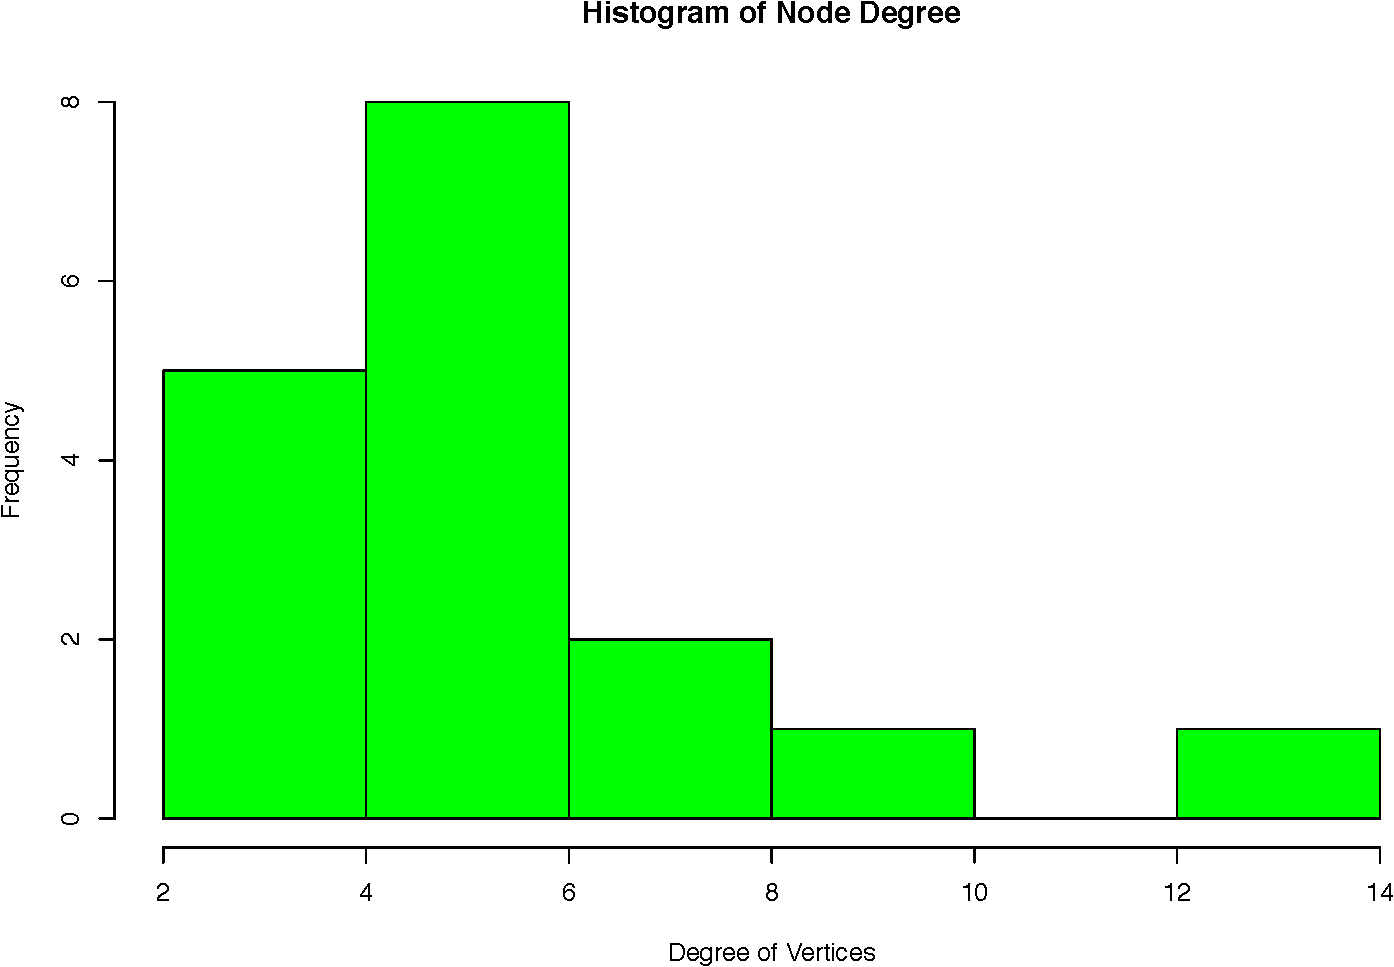
\includegraphics{11_visualisasiSNA_files/figure-beamer/unnamed-chunk-8-1.pdf}
\end{frame}

\hypertarget{network-diagram}{%
\subsection{Network diagram}\label{network-diagram}}

\begin{frame}[fragile]{Network diagram}
\begin{Shaded}
\begin{Highlighting}[]
\FunctionTok{set.seed}\NormalTok{(}\DecValTok{222}\NormalTok{)}
\FunctionTok{plot}\NormalTok{(net,}
     \AttributeTok{vertex.color =} \StringTok{\textquotesingle{}green\textquotesingle{}}\NormalTok{,}
     \AttributeTok{vertext.size =} \DecValTok{2}\NormalTok{,}
     \AttributeTok{edge.arrow.size =} \FloatTok{0.1}\NormalTok{,}
     \AttributeTok{vertex.label.cex =} \FloatTok{0.8}\NormalTok{)}
\end{Highlighting}
\end{Shaded}

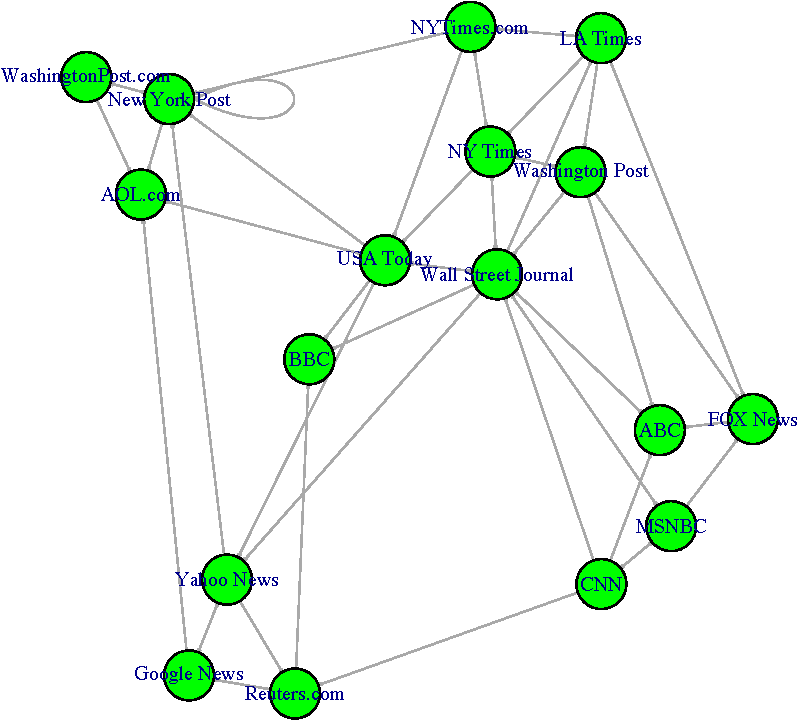
\includegraphics{11_visualisasiSNA_files/figure-beamer/unnamed-chunk-9-1.pdf}
\end{frame}

\hypertarget{highlighting-degrees-layouts}{%
\subsection{Highlighting degrees \&
layouts}\label{highlighting-degrees-layouts}}

\begin{frame}[fragile]{Highlighting degrees \& layouts}
\begin{Shaded}
\begin{Highlighting}[]
\FunctionTok{plot}\NormalTok{(net,}
     \AttributeTok{vertex.color =} \FunctionTok{rainbow}\NormalTok{(}\DecValTok{52}\NormalTok{),}
     \AttributeTok{vertex.size =} \FunctionTok{V}\NormalTok{(net)}\SpecialCharTok{$}\NormalTok{degree}\SpecialCharTok{*}\FloatTok{0.4}\NormalTok{,}
     \AttributeTok{edge.arrow.size =} \FloatTok{0.1}\NormalTok{,}
     \AttributeTok{layout=}\NormalTok{layout.fruchterman.reingold)}
\end{Highlighting}
\end{Shaded}

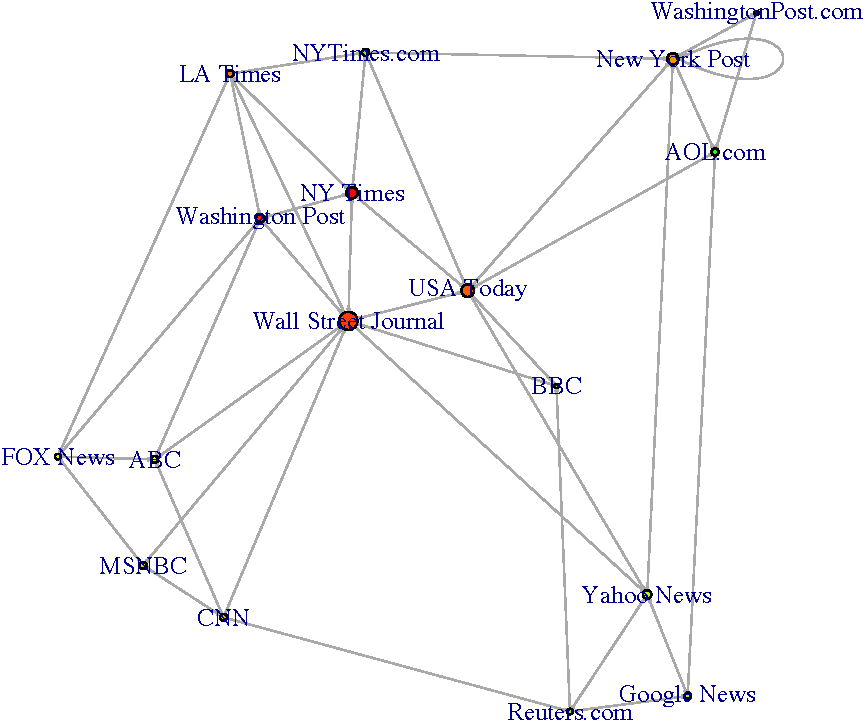
\includegraphics{11_visualisasiSNA_files/figure-beamer/unnamed-chunk-10-1.pdf}

\begin{Shaded}
\begin{Highlighting}[]
\FunctionTok{plot}\NormalTok{(net,}
     \AttributeTok{vertex.color =} \FunctionTok{rainbow}\NormalTok{(}\DecValTok{52}\NormalTok{),}
     \AttributeTok{vertex.size =} \FunctionTok{V}\NormalTok{(net)}\SpecialCharTok{$}\NormalTok{degree}\SpecialCharTok{*}\FloatTok{0.4}\NormalTok{,}
     \AttributeTok{edge.arrow.size =} \FloatTok{0.1}\NormalTok{,}
     \AttributeTok{layout=}\NormalTok{layout.graphopt)}
\end{Highlighting}
\end{Shaded}

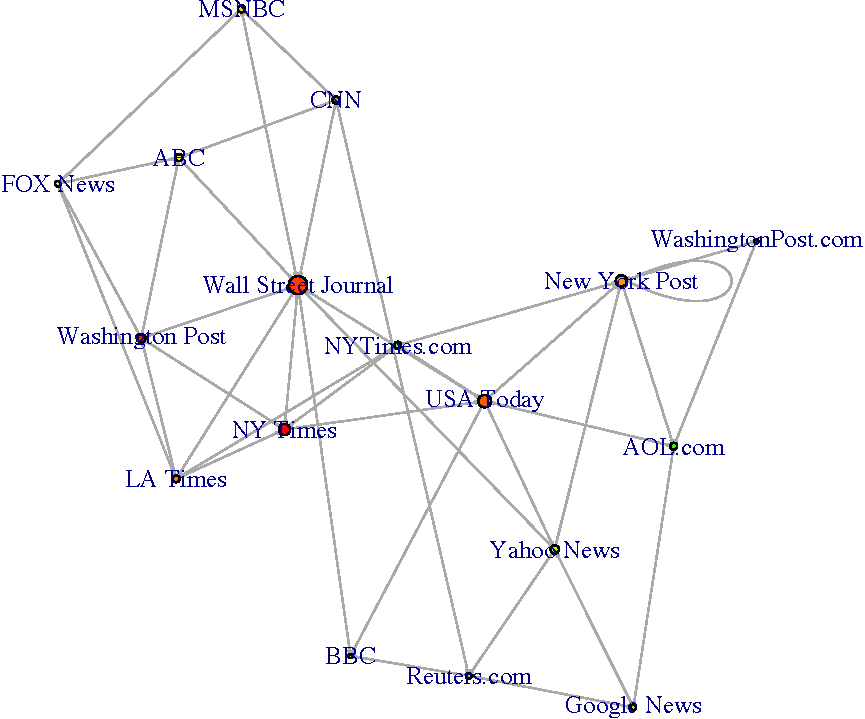
\includegraphics{11_visualisasiSNA_files/figure-beamer/unnamed-chunk-11-1.pdf}

\begin{Shaded}
\begin{Highlighting}[]
\FunctionTok{plot}\NormalTok{(net,}
     \AttributeTok{vertex.color =} \FunctionTok{rainbow}\NormalTok{(}\DecValTok{52}\NormalTok{),}
     \AttributeTok{vertex.size =} \FunctionTok{V}\NormalTok{(net)}\SpecialCharTok{$}\NormalTok{degree}\SpecialCharTok{*}\FloatTok{0.4}\NormalTok{,}
     \AttributeTok{edge.arrow.size =} \FloatTok{0.1}\NormalTok{,}
     \AttributeTok{layout=}\NormalTok{layout.kamada.kawai)}
\end{Highlighting}
\end{Shaded}

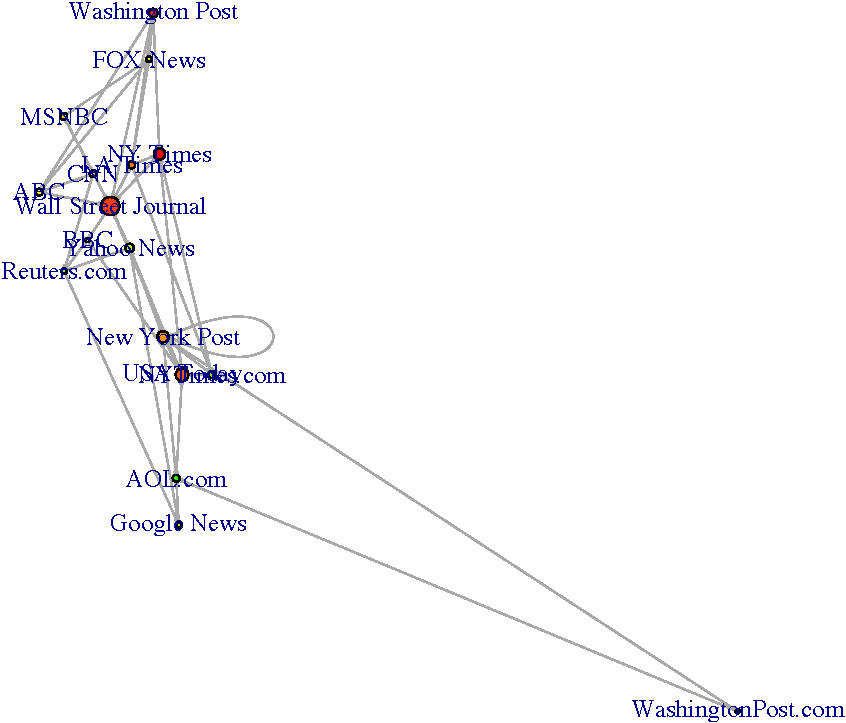
\includegraphics{11_visualisasiSNA_files/figure-beamer/unnamed-chunk-11-2.pdf}
\end{frame}

\hypertarget{hub-and-authorities}{%
\subsection{Hub and Authorities}\label{hub-and-authorities}}

\begin{frame}[fragile]{Hub and Authorities}
Basically, the hub has many outgoing links, and Authorities have many
incoming links.

\begin{Shaded}
\begin{Highlighting}[]
\NormalTok{hs }\OtherTok{\textless{}{-}} \FunctionTok{hub\_score}\NormalTok{(net)}\SpecialCharTok{$}\NormalTok{vector}
\NormalTok{as }\OtherTok{\textless{}{-}} \FunctionTok{authority.score}\NormalTok{(net)}\SpecialCharTok{$}\NormalTok{vector}
\FunctionTok{set.seed}\NormalTok{(}\DecValTok{123}\NormalTok{)}
\FunctionTok{plot}\NormalTok{(net,}
     \AttributeTok{vertex.size=}\NormalTok{hs}\SpecialCharTok{*}\DecValTok{30}\NormalTok{,}
     \AttributeTok{main =} \StringTok{\textquotesingle{}Hubs\textquotesingle{}}\NormalTok{,}
     \AttributeTok{vertex.color =} \FunctionTok{rainbow}\NormalTok{(}\DecValTok{52}\NormalTok{),}
     \AttributeTok{edge.arrow.size=}\FloatTok{0.1}\NormalTok{,}
     \AttributeTok{layout =}\NormalTok{ layout.kamada.kawai)}
\end{Highlighting}
\end{Shaded}

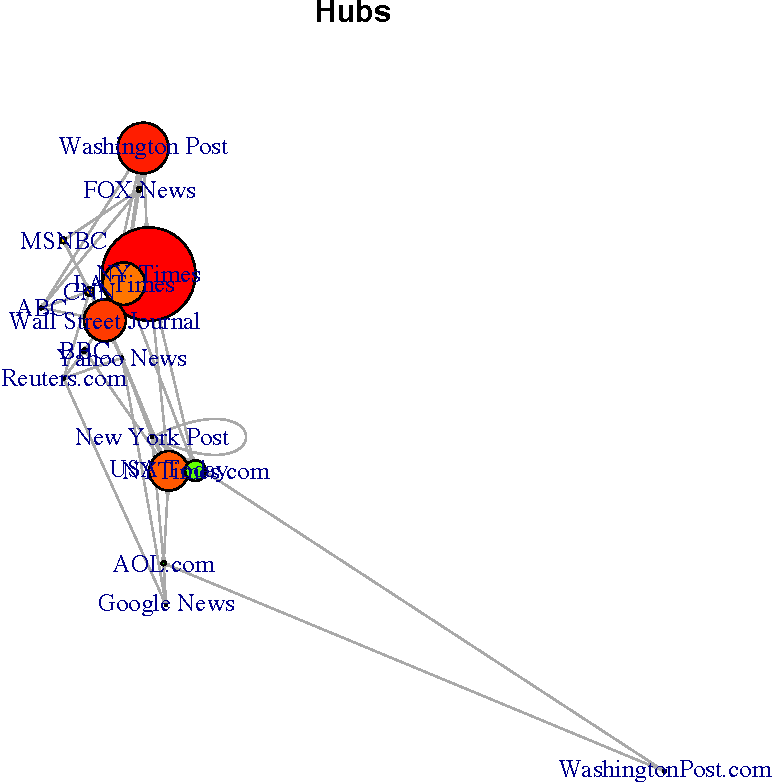
\includegraphics{11_visualisasiSNA_files/figure-beamer/unnamed-chunk-12-1.pdf}

\begin{Shaded}
\begin{Highlighting}[]
\FunctionTok{set.seed}\NormalTok{(}\DecValTok{123}\NormalTok{)}
\FunctionTok{plot}\NormalTok{(net,}
     \AttributeTok{vertex.size=}\NormalTok{as}\SpecialCharTok{*}\DecValTok{30}\NormalTok{,}
     \AttributeTok{main =} \StringTok{\textquotesingle{}Authorities\textquotesingle{}}\NormalTok{,}
     \AttributeTok{vertex.color =} \FunctionTok{rainbow}\NormalTok{(}\DecValTok{52}\NormalTok{),}
     \AttributeTok{edge.arrow.size=}\FloatTok{0.1}\NormalTok{,}
     \AttributeTok{layout =}\NormalTok{ layout.kamada.kawai)}
\end{Highlighting}
\end{Shaded}

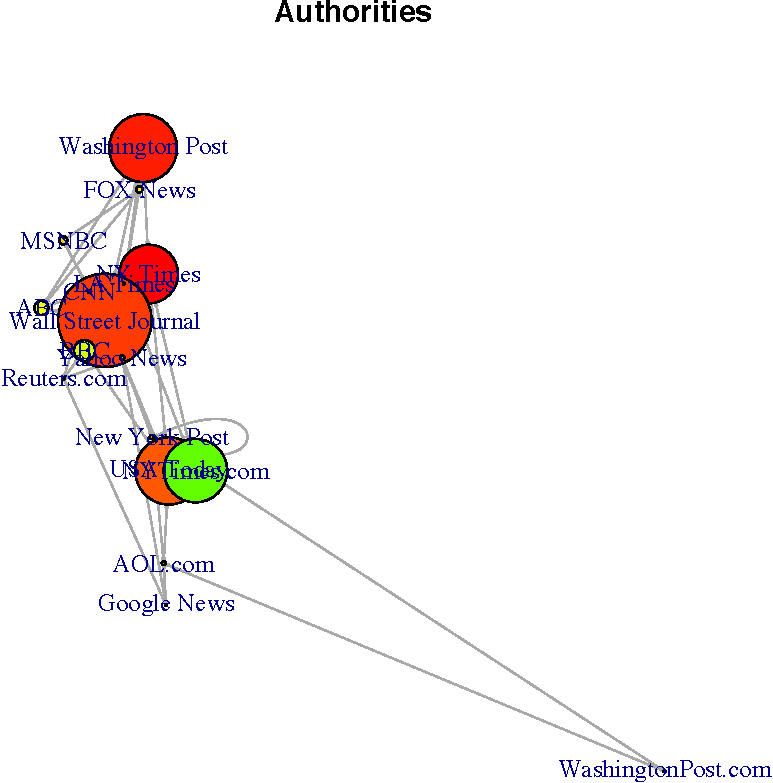
\includegraphics{11_visualisasiSNA_files/figure-beamer/unnamed-chunk-13-1.pdf}
\end{frame}

\hypertarget{community-detection}{%
\subsection{Community Detection}\label{community-detection}}

\begin{frame}[fragile]{Community Detection}
\begin{Shaded}
\begin{Highlighting}[]
\NormalTok{cnet }\OtherTok{\textless{}{-}} \FunctionTok{cluster\_edge\_betweenness}\NormalTok{(net)}
\FunctionTok{plot}\NormalTok{(cnet,}
\NormalTok{     net,}
     \AttributeTok{vertex.size =} \DecValTok{10}\NormalTok{,}
     \AttributeTok{vertex.label.cex =} \FloatTok{0.8}\NormalTok{)}
\end{Highlighting}
\end{Shaded}

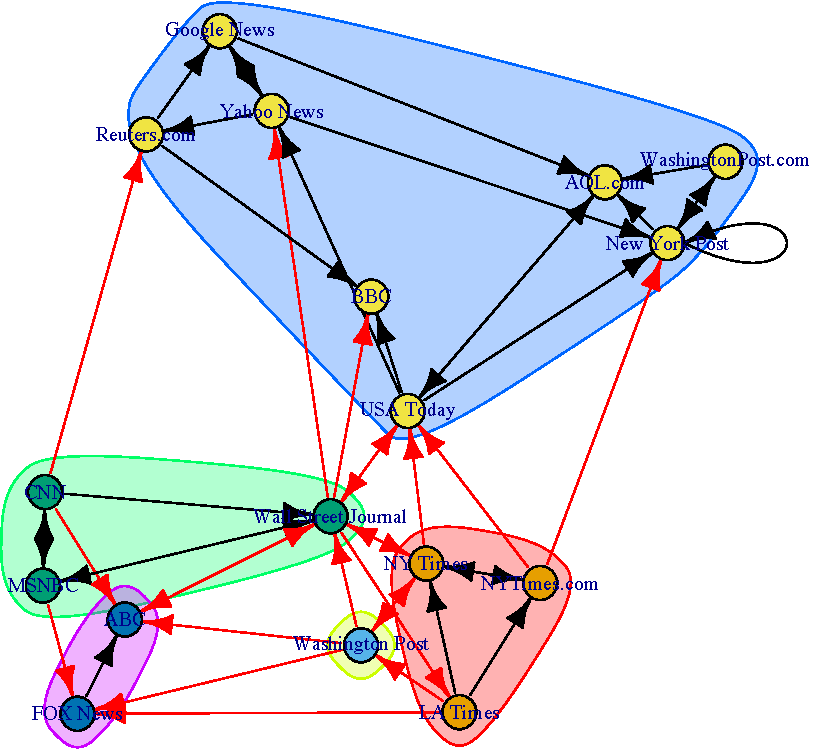
\includegraphics{11_visualisasiSNA_files/figure-beamer/unnamed-chunk-14-1.pdf}
\end{frame}

\hypertarget{analisis-dengan-gephi}{%
\section{Analisis dengan gephi}\label{analisis-dengan-gephi}}

\begin{frame}{Analisis dengan gephi}
Untuk bisa melakukan analisis network di Gephi kita perlu tahu dulu apa
persyaratan yang diperlukan: Dalam konteks ini file seperti apa yang
dibutuhkan di gephi atau perangkat lunak sejenis.
\end{frame}


\section[]{}
\frame{\small \frametitle{Table of Contents}
\tableofcontents}
\end{document}
